\chapter{How to obtain the CRTM}
%===============================

The CRTM source code and coefficients are released as compressed tarballs\footnote{A compressed (e.g. gzip'd) tape archive (tar) file.} via the CRTM ftp site:

\hspace{1cm}\texttt{ftp://ftp.emc.ncep.noaa.gov/jcsda/CRTM/}

A snapshot of that site is shown in figure \ref{fig:ftp_site}. Note that the source code and coefficients can be released separately as updates to either one can occur independently of the other. Also note that additional releases, e.g. beta or experimental branches, are also made available on this ftp site.

\begin{figure}[htb]
  \centering
  \includegraphics[scale=0.5]{graphics/Get/CRTM_ftp_site.eps}
  \caption{The CRTM ftp site contents (as on Jan.29, 2009)}
  \label{fig:ftp_site}
\end{figure}
